\documentclass[a4paper, 12pt]{article}

\usepackage{enumerate}
\usepackage{hyperref}
\hypersetup{
	colorlinks=true,
	linkcolor=blue,
	filecolor=blue,
	urlcolor=blue,
	citecolor=blue,
}
\usepackage{amsmath}
\usepackage{amsthm}
\usepackage{amssymb}
\usepackage[margin=3cm]{geometry}
\usepackage{mathpazo}
\usepackage{url}
\usepackage[labelformat=simple]{subcaption}
\usepackage{tikz}
\usepackage{pgf}
\usepackage{longtable}
\usepackage{multirow}
\usepackage{graphicx}
\usepackage{pgfplots}
\usepackage{cleveref}
\usepackage{amsrefs}
\usepackage{bbm}

\numberwithin{equation}{section}
\numberwithin{figure}{section}

\newtheorem{thm}{Theorem}[section]
\newtheorem*{thm*}{Theorem}
\newtheorem*{con*}{Conjecture}
\newtheorem{lem}[thm]{Lemma}
\newtheorem{prop}[thm]{Proposition}
\newtheorem{cor}[thm]{Corollary}
\newtheorem{lemma}[thm]{Lemma}
\newtheorem{conj}[thm]{Conjecture}

\theoremstyle{definition}
\newtheorem{defn}[thm]{Definition}
\newtheorem{remark}[thm]{Remark}
\newtheorem{ex}[thm]{Example}
\newtheorem{quest}[thm]{Question}
\newtheorem{obs}[thm]{Observation}

\renewcommand{\leq}{\leqslant}
\renewcommand{\geq}{\geqslant}
\newcommand{\N}{\mathbb{N}}
\newcommand{\Z}{\mathbb{Z}}
\newcommand{\Q}{\mathbb{Q}}
\newcommand{\R}{\mathbb{R}}
\newcommand{\C}{\mathbb{C}}
\newcommand{\tr}{\mathrm{t}}

\setcounter{tocdepth}{2}

\allowdisplaybreaks

\title{Geometric Foundations of Data Analysis I}
\author{Joshua Maglione}
\date{\today}

\begin{document}

\maketitle
\tableofcontents

\section{Introduction}

Data analysis and more broadly Data Science is a vast and important field within
Computer Science and Mathematics. At the core, the goal is to make sense of
data, which can be measurements, survey results, behavior patterns, etc. Often
this data comes to us in a very ``high dimension''. That is, there are so many
variables that it is impossible to visualize, and even in low
dimensions, it may not be clear what the best conclusion is based on the
analysis. 

A few references seem to agree that the \textit{total data} on all computers is
something like $\mathbf{10^{23}}$ \textbf{bytes} or about \textbf{100
zettabytes}. While all of this data is not concentrated in one organization, we
still require highly sophisticated tools to make sense of a huge amount of data.
My goal with this course is that you will have a solid foundation with some
standard tools. From this bedrock one could explore more sophisticated methods
of data analysis more easily. 

\bigskip

We will consider four key topics:
\begin{enumerate} 
	\item Least Squares Fitting,
	\item Principal Component Analysis,
	\item Hierarchical Clustering and Persistence,
	\item Nearest Neighbors and the Johnson--Lindenstrauss Theorem
\end{enumerate}

We will be working with the assumption that \textbf{the data we care about is
preserved by orthogonal and linear transformations}. This is not true with all
data---for example, one should not take (proper) linear combinations of people.
However, for data like grams of different kinds of food, this is completely
plausible. This assumption will not always be necessary, but we will just keep
this in mind. 

Half of our time will be spent bringing these ideas to life and getting our
hands dirty. We will be working with Jupyter Notebooks to build familiarity with
the concepts we will discuss. This will be done using Python and standard data
analysis packages like Pandas. 

\section{Least squares fitting}

This method of analysis is both simple and powerful. Like with most things in
mathematics, without some good guiding examples, we can get lost in the
formulas.

\subsection{Build up}\label{sec:build-up}

Suppose we have the following data as seen in \Cref{fig:2d-linear-data}. (Maybe
a company produces parts once per month in lots that vary in size depending on
demand. We write $i$ for the production run, $x_i$ for the lot size, and $y_i$
for the hours of labor.) 

\begin{figure}[h]
	\centering
	\begin{minipage}{0.33\textwidth}
		\centering
		\begin{tabular}{ccc}
			$i$ & $x_i$ & $y_i$ \\ \hline 
			1 & 30 & 73 \\ 
			2 & 20 & 50 \\
			3 & 60 & 128 \\
			4 & 80 & 170 \\
			5 & 40 & 87 \\
			6 & 50 & 108 \\
			7 & 60 & 135 \\
			8 & 30 & 69 \\
			9 & 70 & 148 \\
			10 & 60 & 132 
		\end{tabular}
	\end{minipage}~%
	\begin{minipage}{0.60\textwidth}
		\centering
		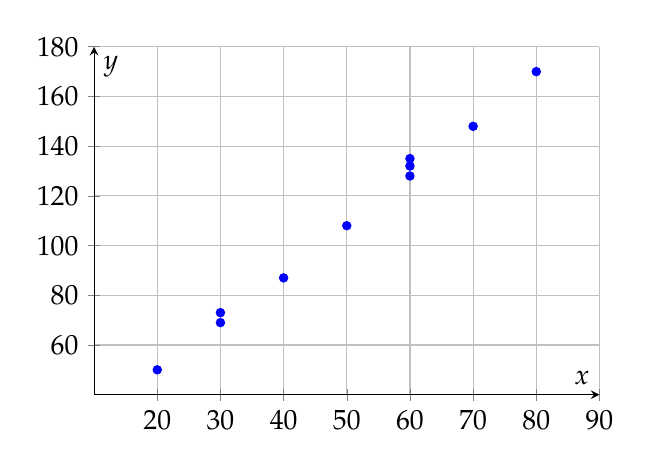
\begin{tikzpicture}
			\begin{axis}[
				xlabel={$x$},
				ylabel={$y$},
				xmin=10, xmax=90,
				ymin=40, ymax=180,
				xtick={10,20,...,90},
				ytick={40,60,...,180},
				grid=both,
				axis lines=middle,
				width=8cm,
				height=6cm,
				]
				\addplot[only marks, mark=*, mark size=1.5pt, color=blue] table {
				30 73
				20 50
				60 128
				80 170
				40 87
				50 108
				60 135
				30 69
				70 148
				60 132
				};
			\end{axis}
		\end{tikzpicture}
	\end{minipage}
	\caption{Data points exhibiting a linear relationship.}
	\label{fig:2d-linear-data}
\end{figure}

It seems clear from the plot that the data fits a geometric pattern---there is a
linear phenomenon. If we try to find the line that is somehow closest to all the
data points, we might draw something like in \Cref{fig:2d-linear-data-line}. 

\begin{figure}[h] 
	\centering
	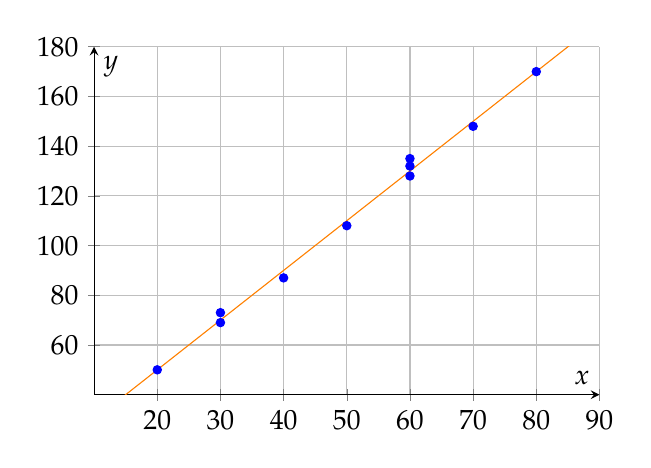
\begin{tikzpicture}
		\begin{axis}[
			xlabel={$x$},
			ylabel={$y$},
			xmin=10, xmax=90,
			ymin=40, ymax=180,
			xtick={10,20,...,90},
			ytick={40,60,...,180},
			grid=both,
			axis lines=middle,
			width=8cm,
			height=6cm,
			]
			\addplot[only marks, mark=*, mark size=1.5pt, color=blue] table {
			30 73
			20 50
			60 128
			80 170
			40 87
			50 108
			60 135
			30 69
			70 148
			60 132
			};
			\addplot[domain=0:90, samples=2, color=orange]{10 + 2*x};
		\end{axis}
	\end{tikzpicture}
	\caption{Line of best fit with data points.}
	\label{fig:2d-linear-data-line}
\end{figure}

Although the line is not a perfect fit, it seems to tell us something about the
relationship between the lots size and the amount of hours. 

\textbf{Questions:}
\begin{itemize}
	\item What makes this line ``better'' than alternatives?
	\item How are we quantifying ``better''? 
	\item Why are we using a line? 
\end{itemize}
We will answer the first question later, probably. Let us consider the question
of quantifying ``better''. Least squares fitting is all about minimizing the
squares of differences between the line and the actual data points. We will make
this precise very soon.

\subsection{Line of best fit}

We know that the equation of a non-vertical line has the form 
\begin{align*}
	y &= b_0 + b_1x.
\end{align*}
If we had $n$ data points of the form $(x_i,y_i)$, we could choose $b_0$ and
$b_1$ to minimize the following sum
\begin{align*}
	S(b_0,b_1) = \sum_{i=1}^n \left(y_i - (b_0 + b_1x_i)\right)^2 .
\end{align*}

We can even solve for these values. Since $S$ is a function in terms of $b_0$
and $b_1$, all possible minima occur when the partial derivatives of $S$ are
$0$. In other words, the minima arise as values $(b_0,b_1)$ such that 
\begin{align*}
	\dfrac{\partial S}{\partial b_0} &= -2\sum_{i=1}^n \left(y_i - (b_0 + b_1x_i)\right) = 0, \\
	\dfrac{\partial S}{\partial b_1} &= -2\sum_{i=1}^n \left(x_iy_i - x_i(b_0 + b_1x_i)\right) = 0.
\end{align*}
These equations are linear equations, so we can solve for these with techniques
from linear algebra. This mean, we need to solve two equations in the unknown
$b_0$ and $b_1$:
\begin{equation}\label{eqn:least-squares-line}
	\begin{split}
		nb_0 + b_1\sum x_i &= \sum y_i, \\
		b_0 \sum x_i + b_1 \sum x_i^2 &= \sum x_iy_i. 
	\end{split}
\end{equation}

Using the data from our example in \Cref{sec:build-up}, we have 
\begin{align*}
	\sum x_i &= 500, & 
	\sum y_i &= 1100, & 
	\sum x_i^2 &= 28400, & 
	\sum x_iy_i &= 61800. 
\end{align*}
Thus, the equations we need to solve are 
\begin{align*}
	10b_0 + 500b_1 &= 1100, \\
	500b_0 + 28400b_1 &= 61800,
\end{align*}
which yield $b_0=10$ and $b_1 = 2$. Going back to the context of the initial
problem: this solution tells us that by increasing the lot size by one, we
expect to increase the labor hours by two. 

\subsubsection{Written as matrices}

Let us write the equations in~\eqref{eqn:least-squares-line} with matrices. This
might seem like overkill at this stage, but it will set us up nicely to
generalize. Let 
\begin{align}\label{eqn:X-Y-B}
	X &= \begin{pmatrix}
		1 & x_1 \\
		1 & x_2 \\
		\vdots & \vdots \\
		1 & x_n
	\end{pmatrix}, & 
	Y &= \begin{pmatrix}
		y_1 \\ y_2 \\ \vdots \\ y_n
	\end{pmatrix}, & 
	B &= \begin{pmatrix}
		b_0 \\ b_1 
	\end{pmatrix}. 
\end{align}
Therefore, the equations in~\eqref{eqn:least-squares-line} are equivalent to the
single matrix equation:
\begin{align}
	X^\tr XB = X^\tr Y.
\end{align}
If $X^{\tr} X$ is invertible, then $B = (X^{\tr}X)^{-1}X^{\tr}Y$.

\subsection{In class exercises pt. I}

\begin{enumerate}
	\item 
	\begin{enumerate} 
		\item With $X$, $Y$, and $B$ as defined in \Cref{eqn:X-Y-B}, show that 
		\begin{align*}
			X^\tr X &= \begin{pmatrix}
				n & \sum x_i \\ \sum x_i & \sum x_i^2
			\end{pmatrix}, & 
			X^\tr Y &= \begin{pmatrix}
				\sum y_i \\ \sum x_iy_i
			\end{pmatrix}. 
		\end{align*}
		\item Show that $X^\tr XB = X^\tr Y$ is equivalent to
		\Cref{eqn:least-squares-line}:
		\begin{align*}
			nb_0 + b_1\sum x_i &= \sum y_i, \\
			b_0 \sum x_i + b_1 \sum x_i^2 &= \sum x_iy_i.
		\end{align*}
	\end{enumerate}
	\item Find a least squares fitting line to the following data and draw in
	the line:
	
	\begin{minipage}{0.3\textwidth}
		\centering 
		\begin{tabular}{ccc}
			$i$ & $x_i$ & $y_i$ \\ \hline
			1 & 1.0 & 1.0 \\ 
			2 & 2.0 & 1.5 \\
			3 & 3.0 & 2.0 \\
			4 & 1.5 & 2.0 \\ 
			5 & 3.5 & 3.0 \\ 
			6 & 3.0 & 4.5 \\ 
			7 & 4.0 & 2.0 \\ 
			8 & 5.0 & 3.5
		\end{tabular}
	\end{minipage}~%
	\begin{minipage}{0.6\textwidth}
		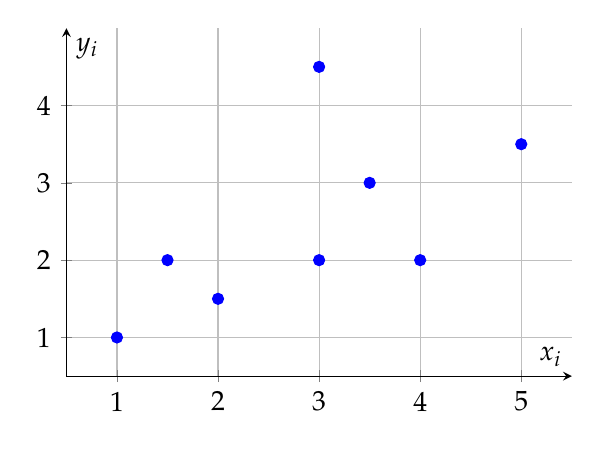
\begin{tikzpicture}
			\begin{axis}[
				xmin=0.5, xmax=5.5,
				ymin=0.5, ymax=5,
				xlabel={$x_i$},
				ylabel={$y_i$},
				xtick={1,2,3,4,5},
				ytick={1,2,3,4},
				grid=both,
				axis lines=middle,
				width=8cm,
				height=6cm,
			]
			\addplot[only marks, mark=*, mark size=2pt, color=blue] table {
				1.0 1.0
				2.0 1.5
				3.0 2.0
				1.5 2.0
				3.5 3.0
				3.0 4.5
				4.0 2.0
				5.0 3.5
			};
			% \addplot[domain=0:90, samples=2, color=orange]{0.94 + 0.52*x};
			\end{axis}
		\end{tikzpicture}
	\end{minipage}

	(Round $b_0$ and $b_1$ to the nearest half integer.)
\end{enumerate}

\subsection{Plane of best fit}

We consider two independent variables and one dependent variable now. Consider
the following data points as given in \Cref{fig:3d-data-points}.

\begin{figure}[h]
	\centering
	\begin{minipage}{0.3\textwidth}
		\centering 
		\begin{tabular}{cccc}
			$i$ & $x_{i1}$ & $x_{i2}$ & $y_i$ \\ \hline
			0 & 278 & 36 & 287 \\
			1 & 252 & 31 & 256 \\
			2 & 344 & 35 & 300 \\
			3 & 134 & 33 & 182 \\
			4 & 215 & 35 & 248 \\
			5 & 261 & 40 & 271 \\
			6 & 131 & 39 & 149 \\
			7 & 463 & 43 & 411 \\
			8 & 167 & 46 & 214 \\
			9 & 298 & 42 & 291 \\
			10 & 230 & 60 & 314 \\
			11 & 293 & 67 & 352 \\
			12 & 290 & 37 & 298 \\
			13 & 271 & 31 & 252 \\
			14 & 385 & 63 & 439 \\
			15 & 354 & 36 & 328
		\end{tabular}
	\end{minipage}~%
	\begin{minipage}{0.6\textwidth}
		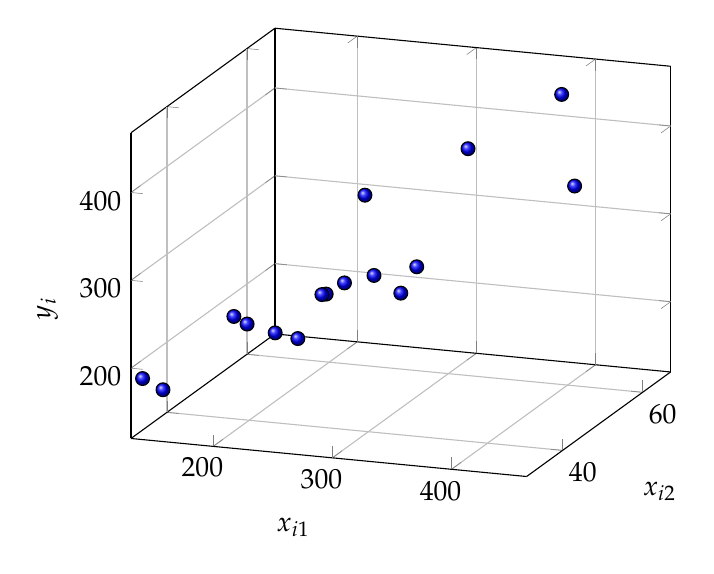
\begin{tikzpicture}
			\begin{axis}[
				view={20}{20}, % Set the view angle
				xlabel=$x_{i1}$,
				ylabel=$x_{i2}$,
				zlabel=$y_i$,
				grid=major,
			]
			% Scatter plot data points
			\addplot3[
				only marks,
				mark=ball,
				mark size=2.5,
			]
			coordinates {
				(278, 36, 287)
				(252, 31, 256)
				(344, 35, 300)
				(134, 33, 182)
				(215, 35, 248)
				(261, 40, 271)
				(131, 39, 149)
				(463, 43, 411)
				(167, 46, 214)
				(298, 42, 291)
				(230, 60, 314)
				(293, 67, 352)
				(290, 37, 298)
				(271, 31, 252)
				(385, 63, 439)
				(354, 36, 328)
			};
			% % Define the equation of the plane: ax + by + cz + d = 0
			% \addplot3[
			% 	surf,
			% 	opacity=0.5,
			% 	faceted color=blue,
			% 	shader=interp,
			% 	domain=200:400,
			% 	domain y=20:60,
			% ] {0.7*x + 2.6*y - 11.3};
			\end{axis}
		\end{tikzpicture}
	\end{minipage}	
	\caption{Data points in $\R^3$.}
	\label{fig:3d-data-points}
\end{figure}

We can put some meaning to these data. For example, suppose a company is selling
a product, and we have 16 populations of people labeled $0$ through $15$. The
values $x_{i1}$ are the population sizes in $100$s of people; the values
$x_{i2}$ are the average yearly income in €$1000$ per capita; and the values
$y_i$ are the number of sales of the product. (There might be dependencies
between population size and average income, but our model treats them as
independent.)

It looks like though there is a plane of best fit for the data---thanks to the
suggestive viewing angle. Our goal is to find a plane, given by 
\begin{align*} 
	y = b_0 + b_1x_1 + b_2x_2. 
\end{align*} 
We can just do what we did last time. That is, for 
\begin{align*}
	X &= \begin{pmatrix}
		1 & x_{11} & x_{12} \\ 
		1 & x_{21} & x_{22} \\
		\vdots & \vdots & \vdots \\
		1 & x_{n1} & x_{n2} 
	\end{pmatrix}, & 
	Y &= \begin{pmatrix}
		y_1 \\ y_2 \\ \vdots \\ y_n
	\end{pmatrix}, & 
	B &= \begin{pmatrix}
		b_0 \\ b_1 \\ b_2
	\end{pmatrix},
\end{align*}
we need to solve for $B$ in the equation
\begin{align*}
	X^{\tr} X B &= X^{\tr} Y .	
\end{align*}
Thus, if $X^{\tr}X$ is invertible, there is a unique $B$, which is equal to
$(X^{\tr}X)^{-1}X^{\tr}Y$. For our example, we have 
\begin{align*}
	X^{\tr}X &= \begin{pmatrix}
		16 &    4366 &     674 \\
		4366 & 1309480 &  187024 \\
		674 &  187024 &   30330
	\end{pmatrix}, & 
	X^{\tr}Y &= \begin{pmatrix}
		4592 \\
		1343400 \\
		200571
	\end{pmatrix}.
\end{align*}
Therefore, the plane of best fit is approximately
\begin{align*}
	y &= -11.3 + 0.7x_1 + 2.6x_2.
\end{align*}
Putting all the data together we have a plane of best fit as seen in
\Cref{fig:plane-and-scatter}.

\begin{figure}[h]
	\centering
	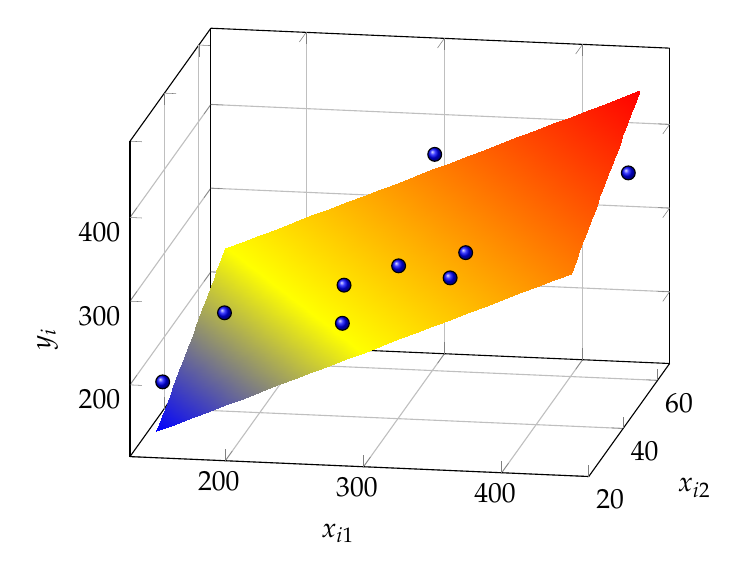
\begin{tikzpicture}
		\begin{axis}[
			view={10}{20}, % Set the view angle
			xlabel=$x_{i1}$,
			ylabel=$x_{i2}$,
			zlabel=$y_i$,
			grid=major,
		]
		% Scatter plot data points
		\addplot3[
			only marks,
			mark=ball,
			mark size=2.5,
		]
		coordinates {
			% (278, 36, 287)
			% (252, 31, 256)
			(344, 35, 300)
			% (134, 33, 182)
			% (215, 35, 248)
			(261, 40, 271)
			(131, 39, 149)
			(463, 43, 411)
			(167, 46, 214)
			(298, 42, 291)
			% (230, 60, 314)
			(293, 67, 352)
			% (290, 37, 298)
			(271, 31, 252)
			% (385, 63, 439)
			(354, 36, 328)
		};
		% Define the equation of the plane: ax + by + cz + d = 0
		\addplot3[
			surf,
			opacity=1,
			shader=interp,
			domain=150:450,
			domain y=20:60,
		] {0.7*x + 2.6*y - 11.3};
		\end{axis}
	\end{tikzpicture}
	\caption{Data points together with the plane of best fit.}
	\label{fig:plane-and-scatter}
\end{figure}

\subsection{Hyperplane of best fit}

Now we go to the general case. Suppose we have $p-1$ independent variables and
$1$ dependent variable, where $p\geq 2$. We assume we have $n$ data points of the form 
\[ 
	\left( x_{i1}, x_{i2}, \dots, x_{i,p-1}, y_1 \right) \in \R^p. 
\] 
The least squares fitting for these data is a hyperplane of the form 
\[ 
	y = b_0 + b_1 x_1 + b_2x_2 + \cdots + b_{p-1}x_{p-1}. 
\] 

To solve for the values $b_i$, we do as we did before. We define matrices 
\begin{align*}
	X &= \begin{pmatrix}
		1 & x_{11} & x_{12} & \cdots & x_{1,p-1} \\
		1 & x_{21} & x_{22} & \cdots & x_{2,p-1} \\
		\vdots & \vdots & \vdots & \ddots & \vdots \\
		1 & x_{n1} & x_{n2} & \cdots & x_{n,p-1} 
	\end{pmatrix}, & 
	Y &= \begin{pmatrix}
		y_1 \\ y_2 \\ \vdots \\ y_n 
	\end{pmatrix}, & 
	B &= \begin{pmatrix}
		b_0 \\ b_1 \\ \vdots \\ b_{p-1}
	\end{pmatrix}. 
\end{align*}
As before, the values we want are given by the equation 
\begin{align}\label{eqn:general-OLS}
	X^{\tr} X B &= X^{\tr} Y.
\end{align}

\subsection{Why \Cref{eqn:general-OLS} works}

The heart of least squares is (Euclidean) distance. The distance between two points $x = (x_1,\dots, x_p)$ and $y=(y_1,\dots, y_p)$ in $\R^p$ is 
\begin{align*}
	d(x, y) = \| x - y \| = \sqrt{(x_1 - y_1)^2 + (x_2 - y_2)^2 + \cdots + (x_p - y_p)^2}. 
\end{align*}
For a vector $v=(v_1,\dots, v_p)\in\R^p$, the \textbf{length} of $v$ is 
\begin{align*}
	\| v \| = d(0, v) = \sqrt{v_1^2 + v_2^2 + \cdots + v_p^2}.
\end{align*}
Recall that the dot product of two (column) vectors $u$ and $v$ is 
\[ 
	u\cdot v = u^{\tr} v = u_1v_1 + u_2v_2 + \cdots + u_pv_p.
\] 
Thus, the length of $v$ is $\| v \| = \sqrt{v\cdot v}$; in other words $\| v\|^2
= v\cdot v$. In addition, if $u\cdot v = 0$, we say that $u$ and $v$ are
\textbf{orthogonal} (or perpendicular).

The goal of least squares is to \textit{minimize distance}; more specifically to
minimize $\|Y - XB\|$. Note that the column vector $Y$ has entries that are the
\textit{actual $y_i$ values}, and the column vector 
\begin{align*}
	XB &= \begin{pmatrix}
		B\cdot (1, x_{11}, x_{12}, \dots, x_{1,p-1}) \\ 
		B\cdot (1, x_{21}, x_{22}, \dots, x_{2,p-1}) \\ 
		\vdots \\
		B\cdot (1, x_{n1}, x_{n2}, \dots, x_{n,p-1}) 
	\end{pmatrix} = \begin{pmatrix}
		b_0 + b_1x_{11} + b_2x_{12} + \cdots + b_{p-1}x_{1,p-1} \\ 
		b_0 + b_1x_{21} + b_2x_{22} + \cdots + b_{p-1}x_{2,p-1} \\ 
		\vdots \\
		b_0 + b_1x_{n1} + b_2x_{n2} + \cdots + b_{p-1}x_{n,p-1}
	\end{pmatrix}
\end{align*}
Therefore, $\| Y - XB \|$ is the square root of a sum of squares of the form 
\begin{align*}
	y_i - b_0 + b_1x_{i1} + b_2x_{i2} + \cdots + b_{p-1}x_{i,p-1}.
\end{align*}
Hence minimizing $\| Y - XB \|$ is the same as minimizing $\| Y - XB \|^2$,
which is a sum of \textit{squares}.

\begin{prop}
	The minimal distance $\| Y - XB \|$ is achieved by solving for $B$ in 
	\[ 
		X^{\tr} X B = X^{\tr} Y.
	\] 
\end{prop}

\begin{proof} 
	Consider the subspace $U = \{Xu ~|~ u\in\R^p\}$ of $\R^n$, and observe that
	our desired solution $XB$ is contained in $U$. Since $\| Y - XB \|$ is
	minimal, we must have that the vector $Y - XB$ is orthogonal to all vectors
	contained in $U$.\footnote{To see why this is true, see Section 6.3.1 of
	\cite{ILA}, which is all about orthogonal decompositions.} That is, $(Xu)
	\cdot (Y - XB) = 0$ for all $u\in\R^p$. In other words, we have for all
	$u\in \R^p$,
	\begin{align*} 
		0 = (Xu)^{\tr} (Y - XB) &= u^{\tr} X^{\tr}(Y - XB) \\
		&= u^{\tr} \left(X^{\tr}Y - X^{\tr}XB\right).
	\end{align*}
	Because $u^{\tr} \left(X^{\tr}Y - X^{\tr}XB\right)=0$ for all $u\in \R^p$,
	it follows that $X^{\tr}Y - X^{\tr}XB=0$. 
\end{proof}

\subsection{In class exercises pt. II}

\begin{enumerate}
	\item Determine $X^{\tr}X$ and $X^{\tr}Y$ with
	\begin{align*}
		X &= \begin{pmatrix}
			1 & x_{11} & x_{12} & \cdots & x_{1,p-1} \\
			1 & x_{21} & x_{22} & \cdots & x_{2,p-1} \\
			\vdots & \vdots & \vdots & \ddots & \vdots \\
			1 & x_{n1} & x_{n2} & \cdots & x_{n,p-1} 
		\end{pmatrix}, & 
		Y &= \begin{pmatrix}
			y_1 \\ y_2 \\ \vdots \\ y_n 
		\end{pmatrix}.
	\end{align*}
	\item Using (1) and by taking partial derivatives of 
	\begin{align}\label{eqn:S-function}
		S(b_0, \dots, b_{p-1}) &= \sum_{i=1}^n (y_i - (b_0 + b_1x_{i1} + b_2x_{i2} + \cdots + b_{p-1}x_{i,p-1}))^2,
	\end{align}
	show that the hyperplane of best fit is obtained by solving
	$X^{\tr}XB=X^{\tr}Y$. (You could try this for $p=3$ first.)
\end{enumerate}

\subsection{Nonlinear fittings}\label{sec:nonlinear-fittings}

Although all of our examples so far have been linear fittings, we will
demonstrate that least squares fittings works in the nonlinear case. What is
important is that we have a candidate equation to fit. In the linear cases, we
tried to fit 
\[ 
	y = b_0 + b_1x_1 + b_2x_2 + \cdots + b_{p-1}x_{p-1}.
\] 

Suppose we have the following data as given in \Cref{fig:nonlinear-data}.
Instead of trying to fit the line $y=b_0+b_1x$, we could try to fit the
parabola: 
\[ 
	y = b_0 + b_1x + b_2x^2. 
\] 
We can treat this the same way as before. Of course the quantities $x$ and $x^2$ are \textit{not} independent, but we can ignore this. Set 
\begin{align*} 
	x_{i1} &= x_i, & x_{i2} &= x_i^2.
\end{align*} 
Therefore, the hyperplane of best fit for the data $(x_{i1}, x_{i2}, y_i)$ will
give us the parabola of best fit. \textit{Try this on your own!} 

\begin{figure}[h]
	\centering
	\begin{minipage}{0.3\textwidth}
		\centering
		\begin{tabular}{cc}
			$x_i$ & $y_i$ \\ \hline
			2.27 & 2.50 \\
			5.06 & -16.13 \\ 
			1.45 & 4.23 \\ 
			5.89 & -22.46 \\
			0.48 & 1.37 \\ 
			-0.22 & 0.86 \\ 
			1.44 & 11.85 \\ 
			-1.77 & -14.71 \\ 
			2.45 & 9.42 \\ 
			-1.54 & -14.07 \\ 
			7.55 & -55.62 \\ 
			1.76 & 4.45 \\ 
			5.16 & -19.56 \\ 
			3.26 & -2.79 \\
			3.23 & 5.20 \\
			0.85 & 8.09
		\end{tabular}
	\end{minipage}~%
	\begin{minipage}{0.65\textwidth}
		\centering
		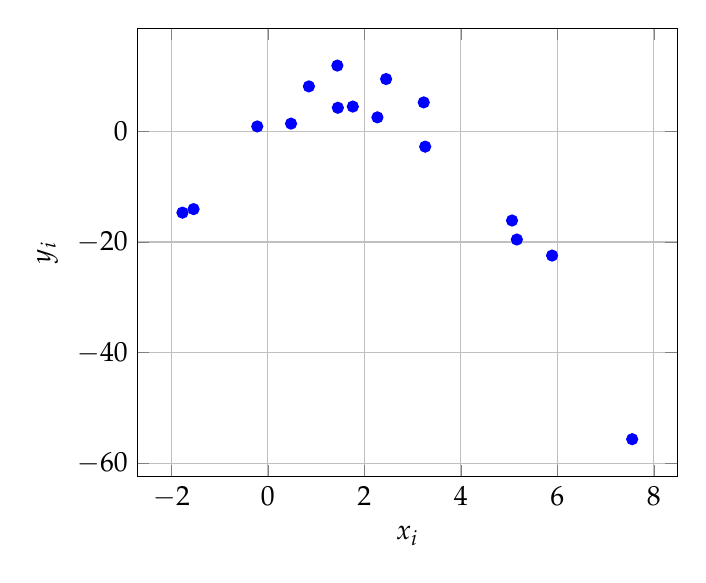
\begin{tikzpicture}
			\begin{axis}[
				xlabel=$x_i$,
				ylabel=$y_i$,
				grid=both,
			]
			\addplot[only marks, mark=*, mark size=2pt, color=blue] coordinates {
				(2.27, 2.50)
				(5.06, -16.13)
				(1.45, 4.23)
				(5.89, -22.46)
				(0.48, 1.37)
				(-0.22, 0.86)
				(1.44, 11.85)
				(-1.77, -14.71)
				(2.45, 9.42)
				(-1.54, -14.07)
				(7.55, -55.62)
				(1.76, 4.45)
				(5.16, -19.56)
				(3.26, -2.79)
				(3.23, 5.20)
				(0.85, 8.09)
			};
			\end{axis}
		\end{tikzpicture}
	\end{minipage}
	\caption{Data points demonstrating a nonlinear relationship.}
	\label{fig:nonlinear-data}
\end{figure}

So one can fit any hypersurface $y=f(x_1,\dots, x_{p-1})$ to the given data. The
function $f$ in this case is called the \textbf{regression function}. This
general method of analysis is known as \textbf{regression analysis}. A few
questions arise:
\begin{itemize}
	\item Which surface is ``best''?
	\item How can we quantify ``best''?
	\item Even in the line case $(p=2)$, how can we quantify how well data fits
	our line? 
\end{itemize}

\subsection{Coefficient of determination ($r^2$ values)}

We are going to make precise how well our hyperplane fits our data. Recall that
hyperplanes can be replaced by hypersurfaces; see \Cref{sec:nonlinear-fittings}.
First we establish some notation. Suppose we have $n$ data points $(x_{i1},
x_{i2}, \dots, x_{i,p-1}, y_i)\in \R^p$. Then we define  
\begin{align*}
	\text{(Fitted value)} & & \widehat{y}_i &= b_0 + b_1x_{i1} + b_2 x_{i2} + \cdots + b_{p-1} x_{i,p-1}, \\
	\text{(Residual)} & & e_i &= y_i - \widehat{y}_i, \\
	\text{(Sample mean)} & & \overline{y} &= \frac{1}{n}\sum_{i=1}^n y_i.
\end{align*}
These yield vectors in $\R^n$ as follows 
\begin{align*}
	\widehat{Y} &= \begin{pmatrix}
		\widehat{y}_1 \\ \vdots \\ \widehat{y}_n
	\end{pmatrix} = XB, & 
	E &= \begin{pmatrix}
		e_1 \\ \vdots \\ e_n
	\end{pmatrix} = Y - \widehat{Y}, & 
	\overline{Y} &= \begin{pmatrix}
		\overline{y} \\ \vdots \\ \overline{y}
	\end{pmatrix} = \overline{y} \begin{pmatrix}
		1 \\ \vdots \\ 1 
	\end{pmatrix}. 
\end{align*}

From our $n$ data points, we have three points in $\R^n$ given by $Y$,
$\widehat{Y}$, and $\overline{Y}$. Three points always lie on a plane, so the
three point determine a triangle on such a plane. What does this triangle look
like? If it is a triangle (and not a line or a single point), then the next
lemma proves it must be a right triangle.

\begin{lem}\label{lem:orthog}
	The vectors $E = Y - \widehat{Y}$ and $\widehat{Y}-\overline{Y}$ are
	orthogonal.
\end{lem}

\begin{proof}
	Suppose $X^{\tr}XB = X^{\tr}Y$. We need to prove two equations. For the
	first, 
	\begin{align*}
		0 &= X^{\tr}(Y - XB) = X^{\tr}(Y - \widehat{Y}) = X^{\tr}E.
	\end{align*}
	Hence, $X^{\tr}E=0$. For the second, 
	\begin{align*}
		\overline{Y}^{\tr}E &= \overline{y} \sum_{i=1}^n (y_i - \widehat{y}_i) \\
		&= \overline{y} \sum_{i=1}^n (y_i - (b_0+b_1x_{i1} + b_2x_{i2} + \cdots + b_{p-1}x_{i,p-1})) \\
		&= -\dfrac{\overline{y}}{2} \cdot \dfrac{\partial S}{\partial b_0} = 0,
	\end{align*}
	where $S$ is defined in \Cref{eqn:S-function}, so $\overline{Y}^{\tr}E=0$.
	Thus, we have 
	\begin{align*}
		(\widehat{Y} - \overline{Y}) \cdot E &= (XB)^{\tr} E - \overline{Y}^{\tr}E = 0. \qedhere
	\end{align*}
\end{proof}

\begin{remark}
	One can simplify the proof for \Cref{lem:orthog} by applying an isometry to
	the data, so that $\overline{y} = 0$. That is, one only needs to prove that
	$E$ and $\widehat{Y}$ are orthogonal.
\end{remark}

The lengths of the differences of the vectors are important and have names: 
\begin{align*} 
	\text{(Sums of Squares Total -- SST)} &: \|Y - \overline{Y} \|^2, \\
	\text{(Sums of Squares Error -- SSE)} &: \| Y - \widehat{Y}\|^2, \\
	\text{(Sums of Squares Regression -- SSR)} &: \| \widehat{Y} - \overline{Y}\|^2 .
\end{align*} 
The value $SST$ measures the \textit{total variability} of the data set. For
example, $\sqrt{SST} = \| Y - \overline{Y} \|$ is the distance from the actual
data $Y$ to the sample mean $Y$. Using the same ideas, we can see that $SSE$
measures the error of our regression and that $SSR$ measures the distance from
our regression to the sample mean. 

\begin{prop}\label{prop:SS-values}
	\[ 
		SST = SSE + SSR. 
	\] 
\end{prop}

\begin{proof}
	Apply \Cref{lem:orthog} and the Pythagorean Theorem:
	\begin{align*} 
		\| Y - \overline{Y} \|^2 &= \| Y - \widehat{Y}\|^2 + \| \widehat{Y} - \overline{Y} \|^2.  \qedhere
	\end{align*} 
\end{proof}

Now we can describe a quantity that measures how good our regression fits the
given data. 

\begin{defn}
	The \textbf{coefficient of determination} (also known as the
	\textbf{$r^2$-value}) is 
	\begin{align*} 
		r^2 &= \dfrac{SSR}{SST} = \dfrac{\|\widehat{Y} - \overline{Y}\|^2}{\| Y - \overline{Y}\|^2} .
	\end{align*} 
\end{defn}

\begin{prop}
	$0\leq r^2 \leq 1$.
\end{prop}

\begin{proof}
	Since each SST and SSR are squares, they are nonnegative. By
	\Cref{prop:SS-values}, we have $0\leq SSR\leq SST$.
\end{proof}

\subsubsection{What do the extremes means?}

The one case where $r^2$ is meaningless is when $SST=0$. This implies both
$SSR=SSE=0$. Moreover, $Y = \overline{Y} = \overline{y} \mathbbm{1}$, where
$\mathbbm{1}$ is the all ones column vector. Hence, every data point $y_i$ is
the same and, therefore, equal to the mean. Let's never return to this case.

We can have $SSR=0$, which is equivalent to $r^2=0$. This implies that $\|
\widehat{Y} - \overline{Y}\|^2= 0$, so that $\widehat{Y} = \overline{Y}$. In
other words, our prediction $\widehat{y}_i$ is just simply the mean. This means
we have not found any relationship between the independent variables and the
dependent variables. 

In the other extreme we have $SSR=SST$, which is equivalent to $r^2=1$. This
implies that $Y = \widehat{Y}$, so the given data lies (exactly) on the surface
given by $y=f(x_1,\dots, x_{p-1})$. That is, the regression function exactly
predicts the data. 

To summarize, when $r^2=0$, we cannot deduce any relationship between the
independent and dependent variables, and when $r^2=1$, we understand completely
the relationship between the independent and dependent variables. Very roughly
speaking, the $r^2$ can be thought of as the ratio of how well the regression
fits the data. 

\subsection{In class exercises pt. III}

\begin{enumerate}
	\item Prove the following.
	\begin{enumerate}
		\item $\| \overline{Y} \|^2 = n\overline{y}$.
		\item $Y \cdot \overline{Y} = \widehat{Y}\cdot \overline{Y} = \| \overline{Y} \|^2$.
		\item $Y\cdot \widehat{Y} = \| \widehat{Y} \|^2$.
	\end{enumerate}
	\item Use (1) to show that 
	\begin{enumerate}
		\item $SST = \|Y\|^2 - \|\overline{Y}\|^2$,
		\item $SSE = \|Y\|^2 - \| \widehat{Y} \|^2$,
		\item $SSR = \| \widehat{Y} \|^2 - \| \overline{Y} \|^2$.
	\end{enumerate}
	\item What are the $r^2$ values for the examples above?
\end{enumerate}



\section{Principal component analysis}

Principal component analysis (PCA) is a power method of analysis that comes
standard in all data science tool kits. With little effort, one can reduce a
complex data set to data that we can more easily see structure. More
specifically, the goal of PCA is to find the ``best'' basis to express the data.
In other words, our initial reference frame may not be the one that best
expresses the structure of our data---PCA is a method to find the ``best''
reference frame.

\subsection{Introducing PCA}

We will start with a toy example, where the analysis is quite simple. Suppose we
have many many data points in $\R^2$ as seen in \Cref{fig:pca-example}.

\begin{figure}[h]
    \centering
    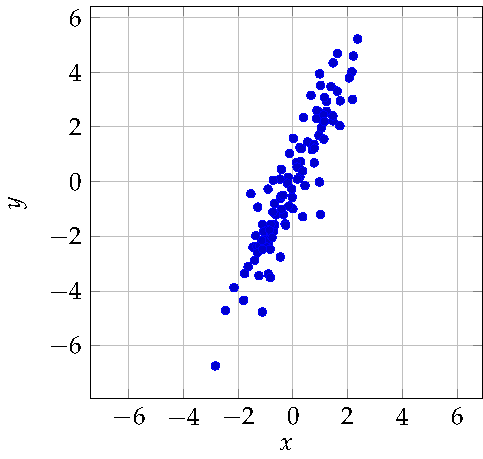
\includegraphics{graphics/pca_example.pdf}
    \caption{Some data in $\mathbb{R}^2$.}
	\label{fig:pca-example}
\end{figure}

Let's assume that our data points live in $\R^m$, so that $m=2$ in
\Cref{fig:pca-example}. Suppose we write those data points in an $m\times n$
matrix $X$. Our current (and default) basis is $\{(1,0, \dots, 0), (0,1, 0,
\dots, 0), \dots, (0,\dots, 0,1)\}$, and we want a basis $\{p_1,p_2, \dots,
p_m\}$ that better reflects the structure of our data. That is, we want an
$m\times m$ matrix $P$, whose rows are the $p_i$, that provides us a better
reference frame. Therefore, we want to transform our data $X$ into a new data
set $Y$ such that 
\[ 
	PX = Y. 
\] 
The columns of $X$ are the ``old'' data, and the columns of $Y$ are the ``new''
data. If the $p_i$ are row vectors and the $x_i$ column vectors, then we want 
\[ 
	PX = \begin{pmatrix} 
		p_1 \\ p_2 \\ \vdots \\ p_m 
	\end{pmatrix} \begin{pmatrix} 
		x_1 & x_2 & \cdots x_n
	\end{pmatrix} = \begin{pmatrix}
		p_1\cdot x_1 & p_1\cdot x_2 & \cdots & p_1\cdot x_n \\
		p_2 \cdot x_1 & p_2 \cdot x_2 & \cdots & p_2 \cdot x_n \\ 
		\vdots & \vdots & \ddots & \vdots \\
		p_m \cdot x_1 & p_m \cdot x_2 & \cdots & p_m \cdot x_n 
	\end{pmatrix}. 
\] 
Thus, if the columns of $Y$ are written $y_i$, we have 
\begin{align}\label{eqn:proj-P}
	y_i &= \begin{pmatrix}
		p_1 \cdot x_i \\ p_2 \cdot x_i \\ \vdots \\ p_m \cdot x_i
	\end{pmatrix}. 
\end{align}

Back to our example from \Cref{fig:pca-example}. We want data with a high
\textit{signal-to-noise} (SNR) ratio as to minimize noise. Assuming our data in
\Cref{fig:pca-example} was collected reasonably well, the direction of largest
variance is the direction of most interesting dynamics. Therefore, the variance
of signal, $\sigma_{\mathrm{s}}^2$, would correspond to the length of the
orange vector in \cref{fig:pca-example2} pointing to the top right, and the
variance of the noise, $\sigma_{\mathrm{n}}^2$, would correspond to the length
of the orange vector pointing to the top left. 

\begin{figure}[h]
    \centering
    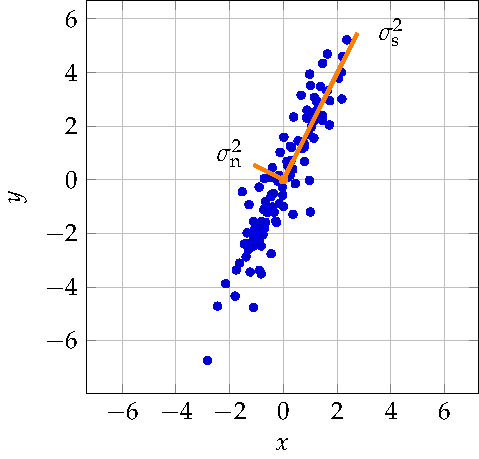
\includegraphics{graphics/pca_example2.pdf}
    \caption{Signal and noise variances represented graphically.}
	\label{fig:pca-example2}
\end{figure}

Note also that in \Cref{fig:pca-example2} knowing the $x$ value gives one a good
approximation for the $y$ value and vice versa. In this case, we might say that
the data has a moderate amount of redundancy, whereas if the data points had a
much higher $r^2$ value to its line of best fit, we would say the data have high
redundancy. (And if the data had a much lower $r^2$ value, we would say the data
have low redundancy.) One of the aims of PCA is to lower redundancy. For the
$2$-dimensional case, this is simple---take the line of best fit, but for
arbitrarily higher dimensions, this is not obvious. 

Suppose we have $n$ measurements 
\[ 
	U = \{u_1, u_2, \dots, u_n\} \qquad \text{ and } \qquad V = \{v_1, v_2, \dots, v_n\}
\] 
\textbf{with mean equal to} $\mathbf{0}$. The \textit{variances} are equal to 
\begin{align*} 
	\sigma_U^2 &= \dfrac{1}{n} \sum_{i=1}^n u_i^2, & \sigma_V^2 &= \dfrac{1}{n} \sum_{i=1}^n v_i^2 .
\end{align*} 
The \textit{covariance} between the data sets $U$ and $V$ is 
\begin{align*}
	\sigma_{UV}^2 &= \dfrac{1}{n} \sum_{i=1}^n u_iv_i.
\end{align*}
The covariance measures the degree of the linear relationship between the two
variables. Thus, a large positive value would imply that the data are positively
correlated, and a large negative value would imply negatively correlated. And
$\sigma_{UV}^2= 0$ if and only if the data $U$ and $V$ are uncorrelated.
Moreover the absolute magnitude of the covariance measures the degree of
redundancy. 

If instead we wrote $u = (u_1, u_2, \dots, u_n)$ and $v= (v_1,v_2, \dots, v_n)$
as row vectors, then 
\begin{align}\label{eqn:vec-covar}
	\sigma_{uv}^2 = \dfrac{1}{n} u v^{\tr}. 
\end{align} 
We generalize from two vectors to $m$ vectors. Write 
\begin{align*}
	X = \begin{pmatrix}
		x_1' \\ x_2' \\ \vdots \\ x_m'
	\end{pmatrix}
\end{align*}
where $x_i'$ is a row vector. Note that the rows of $X$ correspond to
measurements of a particular type, and the columns of $X$ correspond to all
measurements of a particular trail. Using \Cref{eqn:vec-covar}, we define the
\textbf{covariance matrix} of $X$ to be 
\begin{align*} 
	C_X &= \dfrac{1}{n} XX^{\tr} .
\end{align*} 

\begin{lem}
	\begin{enumerate}
		\item The matrix $C_X$ is symmetric. That is, $C_X = C_X^{\tr}$.
		\item The diagonal entries of $C_X$ are variances.
		\item The off-diagonal entries of $C_X$ are covariances.
	\end{enumerate}
\end{lem}

Recall our goal is to find a new (and better) basis $\{p_1, p_2, \dots, p_m\}$.
Namely, we want an invertible matrix $P$ to turn our data $X$ into a data set
$Y$ where we can better understand the structure. If we could do this on the
level of covariance matrices, then we could pick an ideal covariance matrix, one
where the diagonal entries are large in absolute magnitude and where the
off-diagonal entries are small in absolute magnitude. (Variances being high in
magnitude suggest interesting dynamics, and covariances low in magnitude suggest
low redundancy.) In other words, we would like to find a matrix $P$ such that 
\begin{align}\label{eqn:cov-Y}
	C_Y &= \begin{pmatrix}
		\lambda_1 & 0 & \cdots & 0 \\
		0 & \lambda_2 & \cdots & 0 \\
		\vdots & \vdots & \ddots & \vdots \\
		0 & 0 & \cdots & \lambda_m
	\end{pmatrix},
\end{align}
where $Y = PX$. Typically we have $\lambda_1 \geq \lambda_2 \geq \cdots \geq \lambda_m$.

The main work of PCA is finding such a matrix $P$. We will describe how to
construct such a $P$ later, but let us return to our running example.  

The first principal component is in the direction of the largest variance, and
the second principal component is in the orthogonal direction. So in $\R^2$,
this is quite simple. Although we have not given all the data point explicitly,
the covariance matrix is 
\begin{align*}
	C_X &= \begin{pmatrix}
		1.27 & 2.52 \\
		2.52 & 5.95
	\end{pmatrix}.
\end{align*}
The slope of the line in the direction of the highest variance is 1.98, and it
passes through the point $(0,0)$. By rotating and permuting, we get 
\begin{align*}
	P &= \begin{pmatrix}
		0.40 & 0.92 \\ 0.92 & -0.40 
	\end{pmatrix},
\end{align*}
and the graph of the data $Y = PX$ is seen in \Cref{fig:pca-example3}.

\begin{figure}[h]
    \centering
    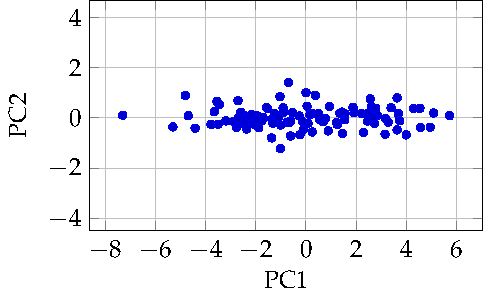
\includegraphics{graphics/pca_example_rotated.pdf}
    \caption{A new basis for our data.}
	\label{fig:pca-example3}
\end{figure}

\begin{remark}
	There is a whole art of scaling data in a pre-processing stage that we will
	not explore in this course. Basically, if one variable ranges between $\pm
	10$ and another $\pm 10^3$, the second variable will bias the process simply
	by its scale. There are many different methods to rescale the data as not to
	lose (too much) information. \textit{Throughout we will assume our data has
	roughly the same scale and not worry about rescaling}, but in practice this
	is an important issue.
\end{remark}

\subsubsection{Assumptions of PCA}

Before we close this introduction to PCA, let us come back to some of the
assumptions we have made along the way. There are three key assumptions we have
made in introducing PCA. We will not focus much on these, but users of PCA
should know that assumptions have been made. These statements may not
necessarily hold for a particular data set. 

\begin{enumerate}
	\item \textit{Linearity.} 
	
	This allows us to reframe the problem as a change of basis problem. 

	\item \textit{Large variance is important (and $SNR>1$).}
	
	This can be a very strong assumption and really needs to take into account
	how the data was collected. 
	
	\item \textit{Principal components are orthogonal.}
	
	This is not always the case, but orthogonality allows us to use linear
	algebra. 
\end{enumerate}

\subsection{In class exercises pt. IV}

\begin{enumerate}
	\item 
	\begin{enumerate}
		\item Show that $C_X$ is symmetric. 
		\item Prove that the diagonal entries of $C_X$ are variances and the
		off-diagonal entries are covariances. 
	\end{enumerate}
	\item Suppose $X$ is an $m\times n$ matrix with sample mean
	$\overline{x}\in\R^m$. Let $X'$ be the shifted data of $X$, so that its
	sample mean is $0$. What is $C_{X'}$ in terms of $X$ and $\overline{x}$?
\end{enumerate}

\subsection{Performing PCA}

At the heart of performing PCA in practice is the following question. Recall
that $C_Y$ is a diagonal matrix; see the discussion around \Cref{eqn:cov-Y}.

\begin{quest} 
	What is the relationship between $C_X$ and $C_Y$ if $Y = PX$? 
\end{quest}

\begin{proof}
	From above, we have
	\begin{align*}
		C_Y &= \dfrac{1}{n} YY^{\tr} = \dfrac{1}{n} (PX)(PX)^{\tr} = P C_X P^{\tr}. \qedhere
	\end{align*}
\end{proof}

In order to perform a PCA, we need to find a matrix $P$ such that $PC_XP^{\tr}$
is diagonal. Importantly, we do not want to change the variances, so we want $P$
to be \textit{distance preserving}; that is, we want $P$ to satisfy
\begin{align}\label{eqn:dist-preserve}
	\| Pv \| &= \| v\|
\end{align}
for all vectors $v\in\R^m$. We say such a matrix $P$ is an \textbf{isometry}. We
can take \Cref{eqn:dist-preserve} and massage it, so that $P$ must satisfy 
\begin{align*}
	v^{\tr} P^{\tr} P v &= (Pv)\cdot (Pv) = v\cdot v = v^{\tr} v
\end{align*}
for all $v\in \R^m$. Since this needs to hold for all vectors, it must hold for
all pairs of basis vectors $(e_i,e_j)$ for all $i,j\in\{1,\dots, m\}$. Thus,
distance preserving is equivalent to $P^{\tr}P = I_m$, but these matrices are
called \textbf{orthogonal}. (Note: pairs of distinct columns of such a matrix
$P$ are pairwise orthogonal. Can you prove this?!) 

Let us bring this back to the equation we established. We want $P$ to be an
orthogonal matrix such that 
\begin{align}\label{eqn:CY-CX}
	C_Y = PC_XP^{\tr} .
\end{align} 
Moreover, we want $C_Y$ to be a diagonal matrix. Since $P^{\tr}P=I_m$, it
follows that $P^{-1} = P^{\tr}$, so using this identity we have 
\begin{align*}
	C_Y &= PC_XP^{-1}.
\end{align*}
Since $C_Y$ is diagonal, this is accomplished through
\textit{eigendecomposition}. Therefore, the rows of $P$ are eigenvectors, and
the diagonal entries of $C_Y$ are eigenvalues.

All the entries of $C_Y$ are \textit{real}, and we know that some matrices have
complex eigenvalues. For example, the matrix 
\begin{align*}
	\begin{pmatrix}
		0 & -1 \\ 1 & 0 
	\end{pmatrix}
\end{align*}
has eigenvalues $i$ and $-i$, for $i=\sqrt{-1}$. \textbf{Is it always possible
to find a real matrix $P$ such that \Cref{eqn:CY-CX} holds?} The answer is
``Yes,'' and we will prove it later. For now, let us assume it is always
possible. 

\medskip

We give a recipe for cooking up the principal components.
\begin{description}
	\item[Given:] $n$ data points $x_i\in\R^m$ (of roughly the same scale),
	\item[Return:] $m$ principal components.
\end{description}
\begin{enumerate}
	\item Compute the mean of each coordinate: $\mu_j = \sum_i x_{ij}$,
	\item Organize the normalised data into a matrix $X = (x_{ij} - \mu_j)$,
	\item Compute the covariance matrix $C_X$ of $X$,
	\item Compute the eigenvectors of $C_X$, and sort them based on their
	eigenvalues: largest is first and smallest is last.
	\item Return the (ordered) orthonormal basis of eigenvectors. 
\end{enumerate}


















\newpage

\begin{bibdiv}
\begin{biblist}
	\bib{ILA}{book}{
		author={Margalit, Dan},
		author={Rabinoff, Joseph},
		title={Interactive Linear Algebra},
		date={2019},
		status={\url{https://textbooks.math.gatech.edu/ila/}},
	}

	\bib{Shlens}{unpublished}{
		author={Shlens, Jonathon},
		title={A tutorial on principal component analysis},
		date={2014},
		status={\href{https://arxiv.org/abs/1404.1100}{\texttt{arXiv:1404.1100}}},
	}
\end{biblist}
\end{bibdiv}

\end{document}